% Template for the submission to:
%   The Annals of Probability           [aop]
%   The Annals of Applied Probability   [aap]
%   The Annals of Statistics            [aos] 
%   The Annals of Applied Statistics    [aoas]
%   Stochastic Systems                  [ssy]
%
%Author: In this template, the places where you need to add information
%        (or delete line) are indicated by {???}.  Mostly the information
%        required is obvious, but some explanations are given in lines starting
%Author:
%All other lines should be ignored.  After editing, there should be
%no instances of ??? after this line.

% use option [preprint] to remove info line at bottom
% journal options: aop,aap,aos,aoas,ssy
% natbib option: authoryear
\documentclass[aoas]{imsart}\usepackage[]{graphicx}\usepackage[]{color}
%% maxwidth is the original width if it is less than linewidth
%% otherwise use linewidth (to make sure the graphics do not exceed the margin)
\makeatletter
\def\maxwidth{ %
  \ifdim\Gin@nat@width>\linewidth
    \linewidth
  \else
    \Gin@nat@width
  \fi
}
\makeatother

\definecolor{fgcolor}{rgb}{0.345, 0.345, 0.345}
\newcommand{\hlnum}[1]{\textcolor[rgb]{0.686,0.059,0.569}{#1}}%
\newcommand{\hlstr}[1]{\textcolor[rgb]{0.192,0.494,0.8}{#1}}%
\newcommand{\hlcom}[1]{\textcolor[rgb]{0.678,0.584,0.686}{\textit{#1}}}%
\newcommand{\hlopt}[1]{\textcolor[rgb]{0,0,0}{#1}}%
\newcommand{\hlstd}[1]{\textcolor[rgb]{0.345,0.345,0.345}{#1}}%
\newcommand{\hlkwa}[1]{\textcolor[rgb]{0.161,0.373,0.58}{\textbf{#1}}}%
\newcommand{\hlkwb}[1]{\textcolor[rgb]{0.69,0.353,0.396}{#1}}%
\newcommand{\hlkwc}[1]{\textcolor[rgb]{0.333,0.667,0.333}{#1}}%
\newcommand{\hlkwd}[1]{\textcolor[rgb]{0.737,0.353,0.396}{\textbf{#1}}}%
\let\hlipl\hlkwb

\usepackage{framed}
\makeatletter
\newenvironment{kframe}{%
 \def\at@end@of@kframe{}%
 \ifinner\ifhmode%
  \def\at@end@of@kframe{\end{minipage}}%
  \begin{minipage}{\columnwidth}%
 \fi\fi%
 \def\FrameCommand##1{\hskip\@totalleftmargin \hskip-\fboxsep
 \colorbox{shadecolor}{##1}\hskip-\fboxsep
     % There is no \\@totalrightmargin, so:
     \hskip-\linewidth \hskip-\@totalleftmargin \hskip\columnwidth}%
 \MakeFramed {\advance\hsize-\width
   \@totalleftmargin\z@ \linewidth\hsize
   \@setminipage}}%
 {\par\unskip\endMakeFramed%
 \at@end@of@kframe}
\makeatother

\definecolor{shadecolor}{rgb}{.97, .97, .97}
\definecolor{messagecolor}{rgb}{0, 0, 0}
\definecolor{warningcolor}{rgb}{1, 0, 1}
\definecolor{errorcolor}{rgb}{1, 0, 0}
\newenvironment{knitrout}{}{} % an empty environment to be redefined in TeX

\usepackage{alltt}

\usepackage{amsthm,amsmath,natbib}
\RequirePackage[colorlinks,citecolor=blue,urlcolor=blue]{hyperref}

% provide arXiv number if available:
\arxiv{arXiv:1601.05788}

% put your definitions there:
\startlocaldefs
\usepackage[hang, small,labelfont=bf,up,textfont=it,up]{caption} % Custom captions under/above floats in tables or figures
\usepackage{subcaption}
\usepackage{lineno}
\modulolinenumbers[5]

\usepackage{dcolumn}
\newcolumntype{d}[1]{D{.}{.}{#1}}

\usepackage{pdflscape}

\newcommand{\hh}[1]{{\color{magenta} #1}}
\newcommand{\eh}[1]{{\color{blue} #1}}
\newcommand{\ac}[1]{{\color{darkgreen} #1}}

\endlocaldefs
\IfFileExists{upquote.sty}{\usepackage{upquote}}{}
\begin{document}

\begin{frontmatter}

% "Title of the paper"
\title{Supplement to Automatic Matching of Bullet Lands}
\runtitle{Supplement: Automatic Matching of Bullet Lands}

% indicate corresponding author with \corref{}
\begin{aug}
\author{\fnms{Eric} \snm{Hare}\corref{}\ead[label=e1]{erichare@iastate.edu}\thanksref{m1}},
\author{\fnms{Heike} \snm{Hofmann}\ead[label=e2]{hofmann@iastate.edu}\thanksref{m1}}
\and
\author{\fnms{Alicia} \snm{Carriquiry}\ead[label=e3]{alicia@iastate.edu}\thanksref{m1}}

\affiliation{Iowa State University\thanksmark{m1}}

\runauthor{E. Hare et al.}
\end{aug}

\end{frontmatter}

\linenumbers
\tableofcontents
\newpage


\section{Cylindrical Fit}\label{supp:cylindrical}
Figure~\ref{fig:fixedX} shows the  profile of surface measurements of bullet 1-5 at a fixed height. The smooth line on top is a circle, with estimated radius and center. The details of this fit are given below:
%
\begin{figure}[hbtp]
  \centering
\begin{knitrout}
\definecolor{shadecolor}{rgb}{0.969, 0.969, 0.969}\color{fgcolor}
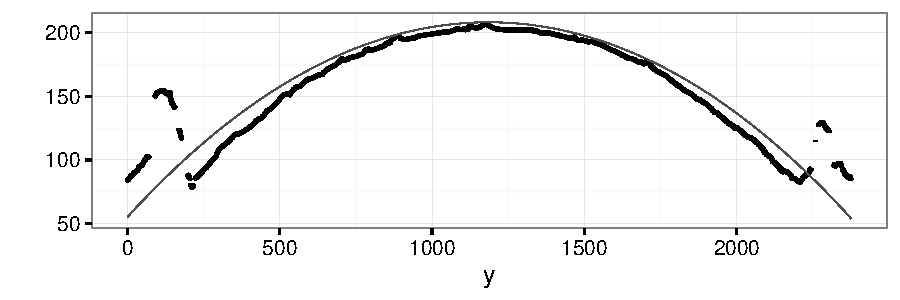
\includegraphics[width=0.5\textwidth]{figure/fixedX-1} 

\end{knitrout}
\caption{\label{fig:fixedX}Side profile of the surface measurements (in $\mu m$) of a bullet land at a fixed height of $x$. Note that the global features dominate any deviations, corresponding to the individual characteristics of striation marks.}
\end{figure}

%One reasonable approach is to fit a circle to the curve and compute the residuals from this fit.

Assume that $n$ data points are given in the form of data tuples $(x_1, y_1)$, $(x_2, y_2)$, $...$, $(x_n, y_n)$ that are (approximately) located on a circle. We want to estimate the location of the center and radius of the best fitting circle using a least squares approach.

We minimize the following expression:
\begin{equation}\label{eq:circle}
D = \sum_{i=1}^n \left( r^2 - (x_i-a)^2 - (y_i-b)^2 \right)^2,
\end{equation}
by differentiating $D$ with respect to $r, a,$ and $b$:
let us assume that $x_i$ and $y_i$ are centered (i.e. $\sum x_i = \sum_i y_i = 0$). Note, if they are not, make a note of the current means, subtract them now and add them to $(\hat{a}, \hat{b})$ at the end. 

\noindent
The  derivate of $D$ with respect to $r$ is:
\begin{eqnarray*}
\frac{d}{dr} D &=& 2 \sum_i \left( r^2 - (x_i-a)^2 - (y_i-b)^2 \right) 2 r = \\
&=& 4 r \left( n r^2 - \sum_i (x_i-a)^2 - \sum_i(y_i-b)^2 \right).
\end{eqnarray*}
At the minimum:
\begin{equation}\label{eq:rmin}
\frac{d}{dr} D = 0 \stackrel{r \neq 0}{\iff} nr^2  = \sum_i (x_i-a)^2 + \sum_i(y_i-b)^2.
\end{equation}
%
%
The  derivative of $D$ with respect to $a$ is:
\begin{eqnarray*}
\frac{d}{da} D &=& 2 \sum_i \left( r^2 - (x_i-a)^2 - (y_i-b)^2 \right) 2 (x_i - a) = \\
&=& -4 \left[ a \cdot nr^2 + \sum_i (x_i - a)^3  + \sum_i (x_i - a) (y_i - b)^2 \right].
\end{eqnarray*}
Using (\ref{eq:rmin}) for $nr^2$  in the equation above we get:
\begin{eqnarray*}
\frac{d}{da} D &=& -4 \left[  \sum_i a(x_i-a)^2 +  \sum_i a(y_i-b)^2  + \right. \\
&& \phantom{-4 \ \ } \left . \sum_i (x_i - a)^3  + \sum_i (x_i - a) (y_i - b)^2 \right]  = \\
&=& -4 \left[ \sum_i (x_i-a)^2 (a + x_i - a)  + \right.\\
&& \phantom{-4 \ \ } \left .\sum_i (x_i - a + a) (y_i - b)^2 \right] = \\
&=& -4 \left[ \sum_i (x_i-a)^2 x_i   + \sum_i x_i  (y_i - b)^2 \right] 
\stackrel{\begin{array}{c}\sum_i x_i = 0\\
\sum_i y_i = 0\end{array}}{=} \\
&=& -4 \left[ \sum_i x_i^3   + \sum_i x_i y_i^2  - 2a s_{xx} - 2b s_{xy} \right],
\end{eqnarray*}
where $s_{xx} = \sum_i x_i^2, s_{xy} = \sum_i x_i y_i$ and $s_{yy} = \sum_i y_i^2$.

\noindent
Likewise, we get for the derivative of $D$ with respect to $b$:
\begin{eqnarray*}
\frac{d}{db} D &=& -4 \left[ \sum_i y_i^3   + \sum_i x_i^2 y_i - 2a s_{xy} - 2b s_{yy} \right].
\end{eqnarray*}
To find the minimum we therefore get a system of two linear equations in $a$ and $b$:
\begin{eqnarray*}
2 s_{xx} a + 2 s_{xy} b = c_1 && \text{ with } c_1 = \sum_i x_i^3 + x_i y_i^2 \\
2 s_{xy} a + 2 s_{yy} b = c_2 &&\text{ with } c_2 = \sum_i x_i^2 y_i + y_i^3.
\end{eqnarray*}
The solution to the system is:
\begin{eqnarray*}
\hat{a} &=& \frac{c_1 s_{yy} - c_2 s_{xy}}{2 s_{xx} s_{yy} - 2 s_{xy}^2},\\
\hat{b} &=& \frac{c_2 s_{xx} - c_1 s_{xy}}{2 s_{xx} s_{yy} - 2 s_{xy}^2}, \text{ and}\\
\hat{r^2} &=& \frac{1}{n}s_{xx} + \frac{1}{n}s_{yy} + \hat{a}^2 + \hat{b}^2.
\end{eqnarray*}


The scatterplot in Figure~\ref{fig:residual} shows the residuals of such a fit.
In this instance, the radius is estimated as $\hat{r} = 4666.49\mu m = 4.67mm$ and the land covers about 29.5 degrees.  Both of these estimates are consistent with a 9 mm bullet fired by a Ruger P-85.
The residuals are dominated, as expected, by the grooves, which show up as large positive residuals. For a profile at height $x = 100\mu m$ there is a residual circular structure that does not show up for all signatures. 

\begin{figure}[hbtp]
  \centering
\begin{subfigure}[b]{.49\textwidth}\centering
\caption{\label{fig:residuala}Residual structure at height $x = 1.5625\mu m$ (bottom of the bullet).}
\begin{knitrout}
\definecolor{shadecolor}{rgb}{0.969, 0.969, 0.969}\color{fgcolor}
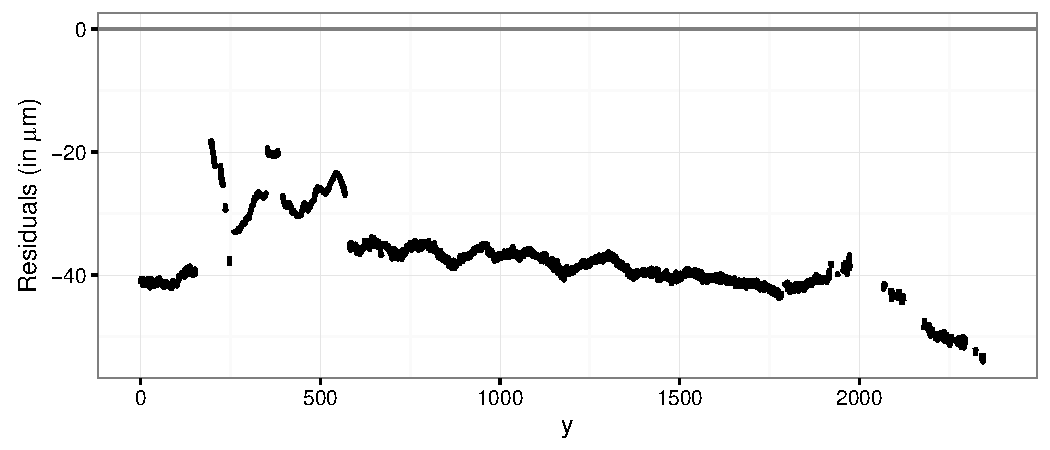
\includegraphics[width=\textwidth]{figure/residual2-1} 

\end{knitrout}
\end{subfigure}    
\begin{subfigure}[b]{.49\textwidth}\centering
\caption{\label{fig:residualb} Residual structure at height $x = 100.00\mu m$}
\begin{knitrout}
\definecolor{shadecolor}{rgb}{0.969, 0.969, 0.969}\color{fgcolor}
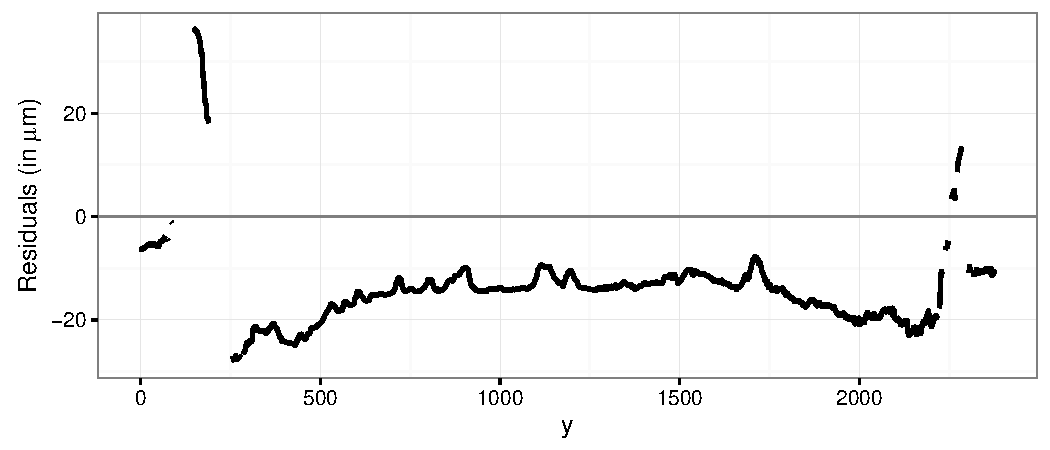
\includegraphics[width=\textwidth]{figure/residual-1} 

\end{knitrout}
\end{subfigure}
\caption{\label{fig:residual} Residual structure of circular fits at two different cross sections. Both residual plots show systematic structures, indicating that a circular fit is not entirely appropriate.}
\end{figure}

A single cylinder as a fit is unlikely to be a particularly good fit, because there seem to be quite massive deformations in the vertical direction. Even when we fit a circle at each distinct height of the bullet, as in Figure~\ref{fig:circlefits}, this does not address all of these issues. While the wider circumference at the base of the bullet can be resolved by individual circular fits, the systematic residual structure in Figure~\ref{fig:residualb} stays the same.





\begin{figure}[hbtp]
  \centering
\begin{knitrout}
\definecolor{shadecolor}{rgb}{0.969, 0.969, 0.969}\color{fgcolor}
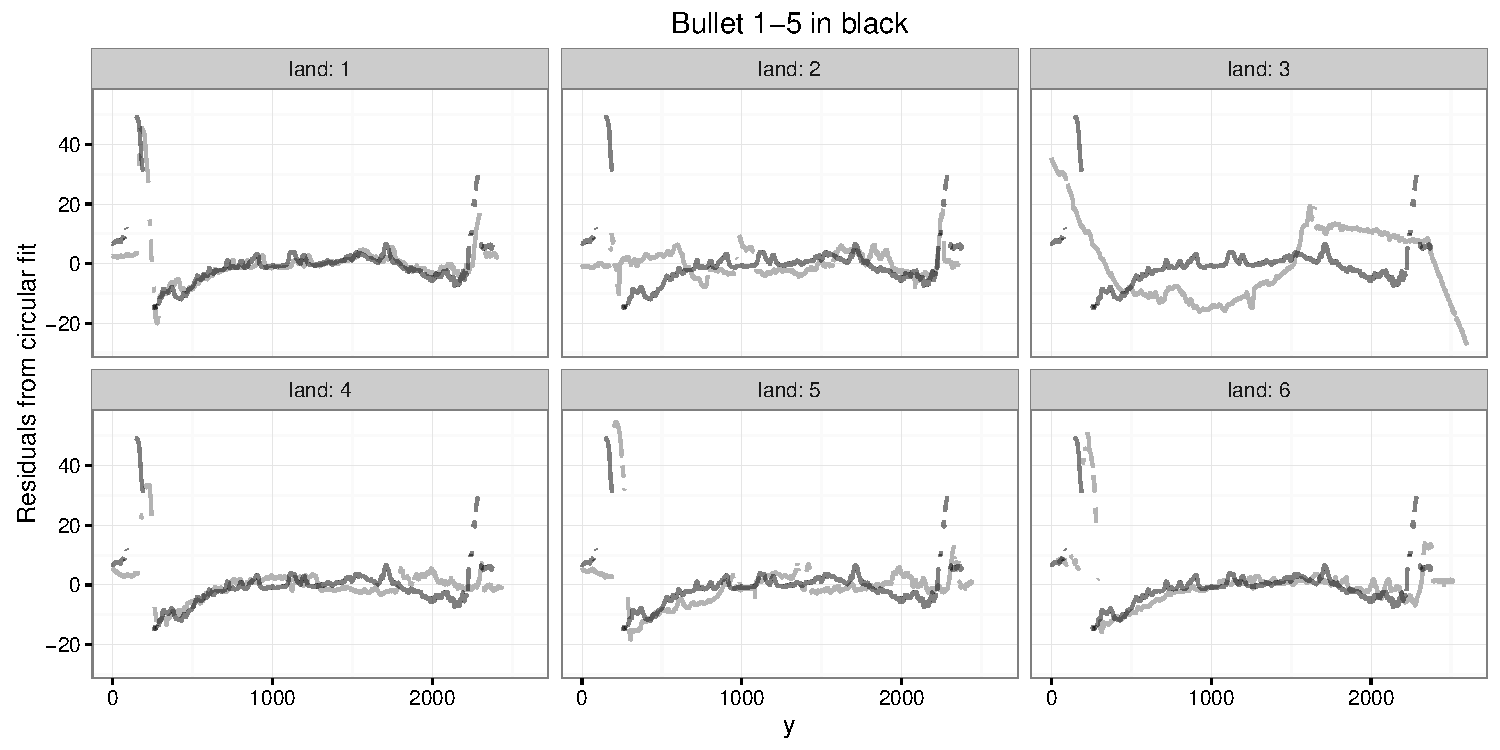
\includegraphics[width=\textwidth]{figure/circlefits-1} 

\end{knitrout}
\caption{Circular fit to the signature of each land of bullet 2, with signature from bullet 1-5 overlaid.\label{fig:circlefits} The signature of bullet 1-5 matches best with bullet 2-1.}
\end{figure}

\newpage
\section{Assessing cross-correlation between signatures at multiple levels of height}\label{supp:ccf}

Figure~\ref{fig:crosscuts} shows a sequence of signatures for bullet 1-5 (barrel 1) that are taken at heights 50$\mu m$ apart, between 150$\mu m$  and 400$\mu m$. These are compared to the signature at a height of 100$\mu m$. Initially, this comparison constitutes an almost perfect match between the two signatures. However, the match quickly deteriorates with increasing distance between the heights at which signatures are extracted.  Only if signatures are from heights  within 150$\mu m$ do we get a good visual match even when we know that the same bullet surface is being used. 
Given that we have to expect some variation in nominally the same height values due to (manual) alignments in microscopes, we should take height values into account in the automatic matching routine by evaluating matches at several heights. 
\begin{figure}[hbtp]
  \centering
\begin{knitrout}
\definecolor{shadecolor}{rgb}{0.969, 0.969, 0.969}\color{fgcolor}
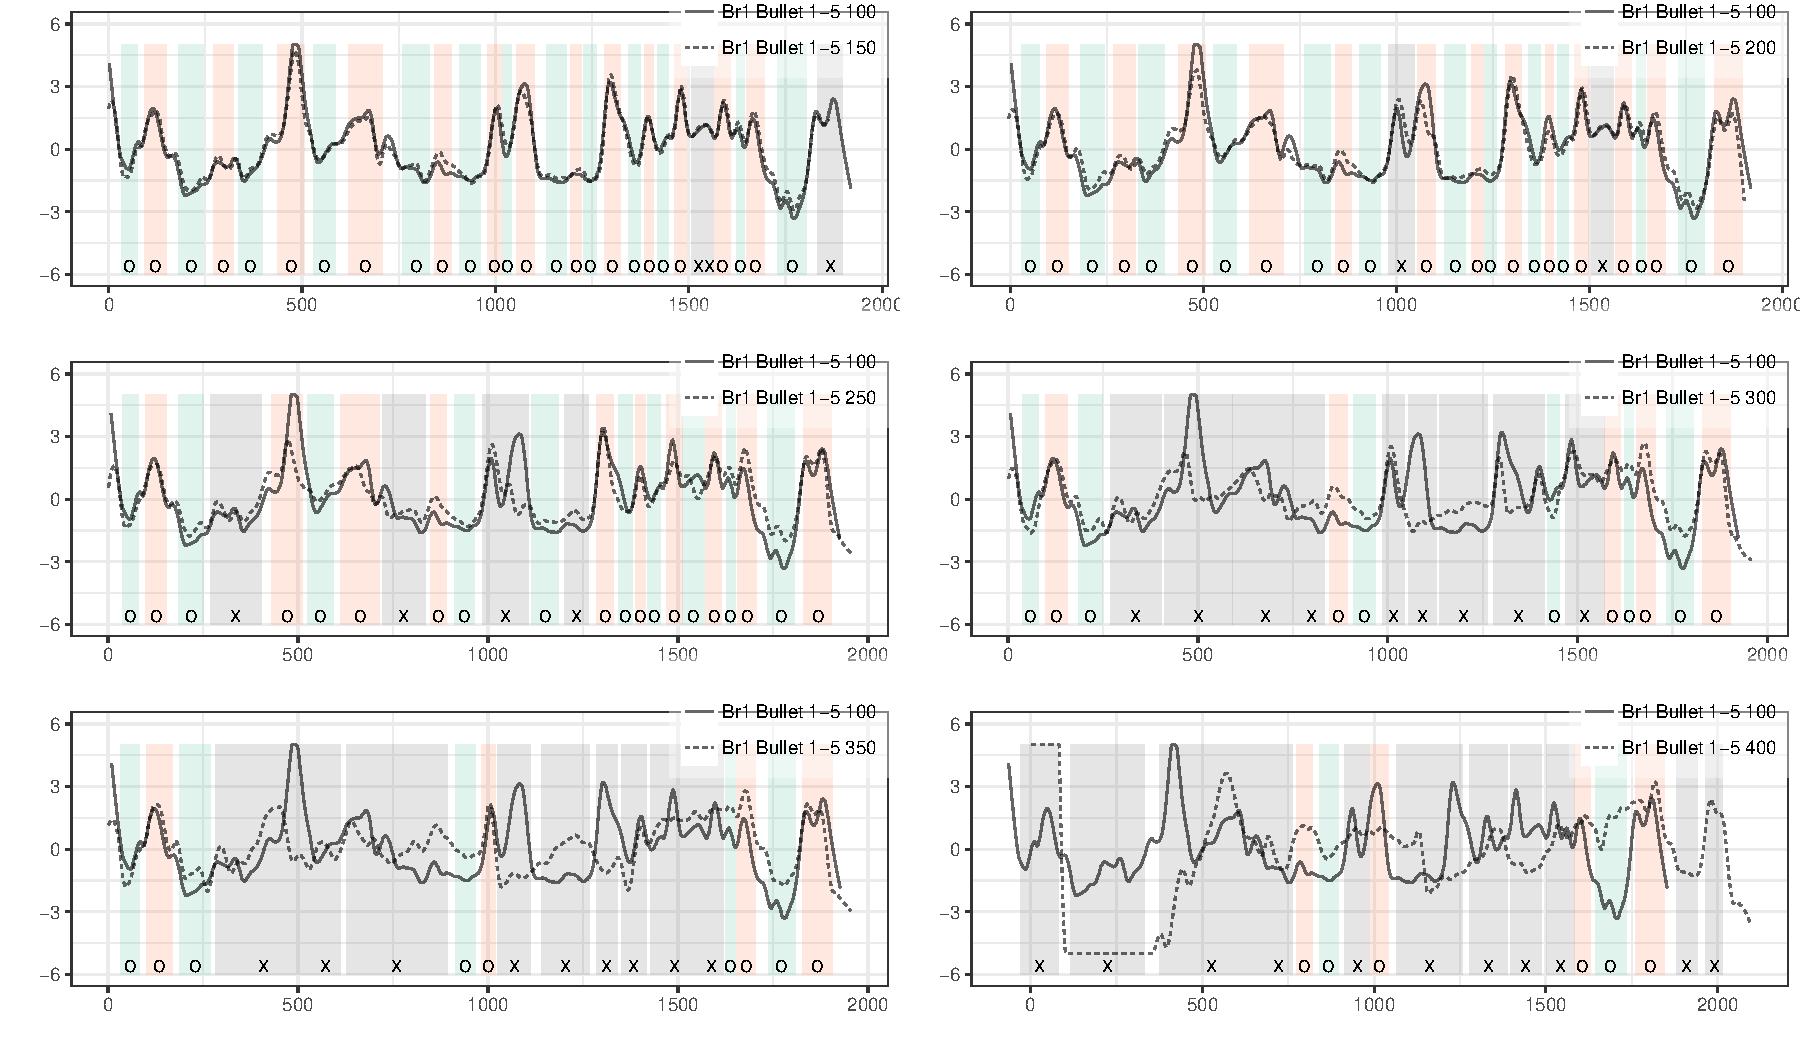
\includegraphics[width=\textwidth]{figure/crosscuts-vary-1} 

\end{knitrout}
\caption{\label{fig:crosscuts}Overview of the variations in the signatures at different heights. The signature extracted at $x = 100\mu m$ is compared to signatures at every 50$\mu m$. With every step away from the original height, the number of differences between the signatures increases; the number of maximum CMS decreases from initially 22 to  four or fewer at a height of $x = 300\mu m$ and above. }
\end{figure}

\newpage
\section{Signature intensities}\label{supp:bulletbottom}

%
Figure~\ref{fig:overview} shows an overview of the signatures at different heights on a single bullet. 
\begin{figure}[hbtp]
\begin{knitrout}
\definecolor{shadecolor}{rgb}{0.969, 0.969, 0.969}\color{fgcolor}
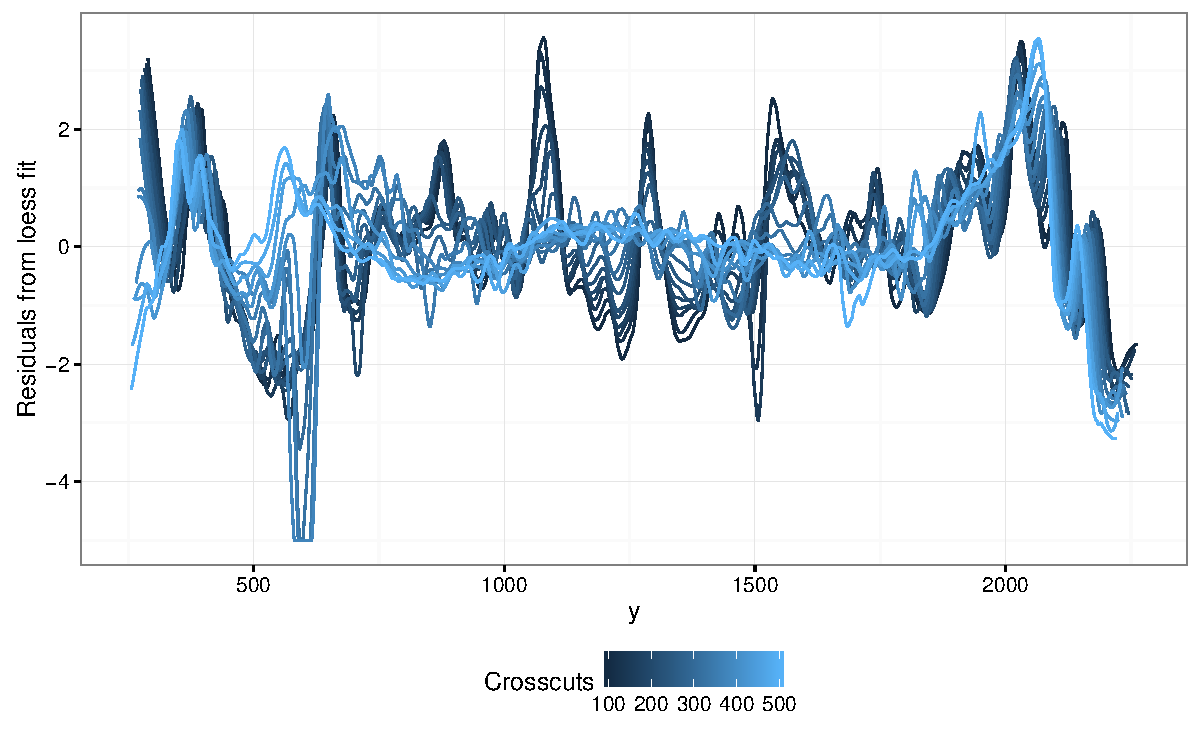
\includegraphics[width=0.7\textwidth]{figure/one-bulletland-sd-1} 

\end{knitrout}
\caption{\label{fig:overview}Signatures of the same bullet at different heights.  With increasing height, peaks and valleys are less pronounced, resulting in a smaller standard deviation.}
\end{figure}
At larger heights  individual characteristics become less distinctive, making true matches to other bullets harder. The pattern of decreasing peaks and valleys is generally true for  bullet lands, as can be seen in Figure~\ref{fig:sds}. 
%
\begin{figure}[hbtp]
\centering
\begin{knitrout}
\definecolor{shadecolor}{rgb}{0.969, 0.969, 0.969}\color{fgcolor}\begin{kframe}


{\ttfamily\noindent\itshape\color{messagecolor}{\#\# `geom\_smooth()` using method = 'gam'}}\end{kframe}
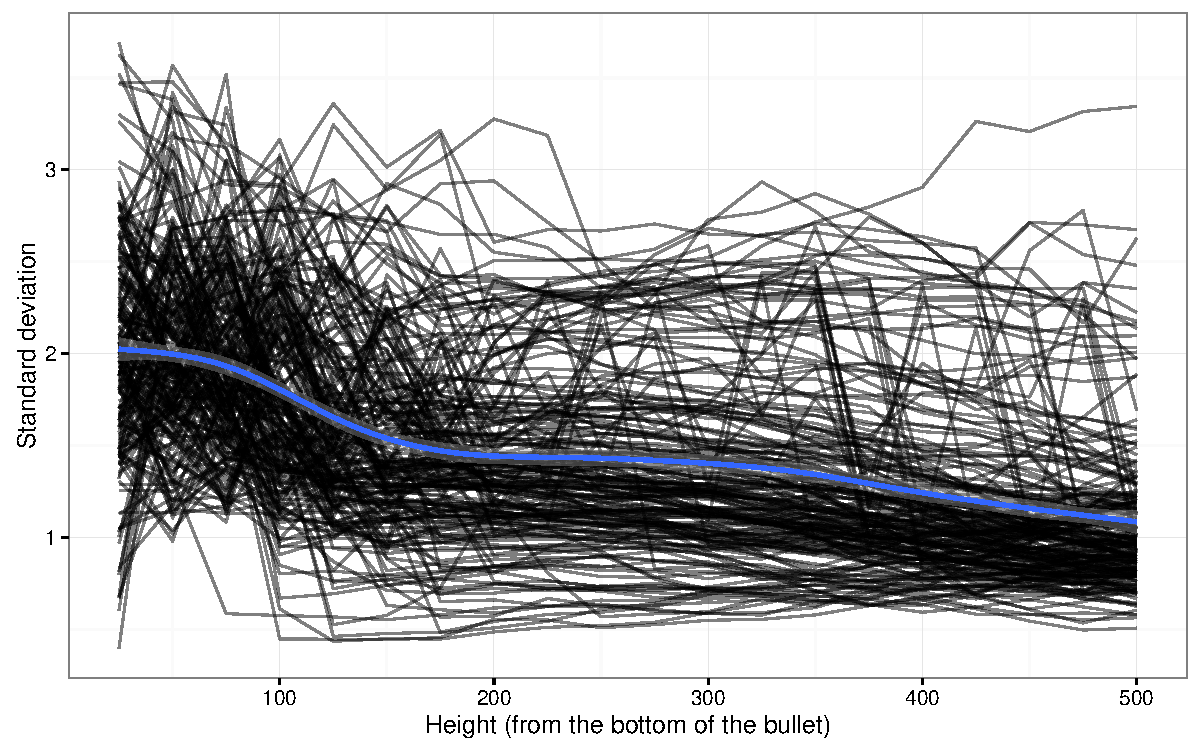
\includegraphics[width=.7\textwidth]{figure/crosscuts-sd-1} 

\end{knitrout}
\caption{\label{fig:sds}Standard deviation reduces as height increase.}
\end{figure}
Figure~\ref{fig:sds} shows that the amount of standard deviation of a signature decreases on average for all bullet lands at larger heights.
This makes standard deviation of a signature one measure to quantify the extent to which a signature is expressed. For identifying matches we should therefore use the lowest height to extract a bullet's signature once a stable surface region is detected. This is in accordance with current standard practice \citep{afte:1992}.

%\newpage
\section{Complete evaluation of the Hamby study}\label{supp:extended}
One way to expand the use of the James Hamby study is to not only match all of the unknown bullet lands against the known bullet lands, but to compare every land against every other land. This effectively doubles the number of comparisons from 10,384 pairwise comparisons of usable bullet lands to 21,115 $\left[= (118+88)\cdot 205/2\right]$ comparisons by adding another 10,731 bullet land comparisons made up of known-to-known and unknown-to-unkown comparisons. 

When we predict the new 10,731 comparisons using the random forest based on the previously considered 10,384 known-unknown comparisons, we encounter 18 false negatives and 9 false positives, corresponding to an actual false error rate of 0.19 and a false positive rate of 0.00085, which is close to the random forest's estimated OOB error rates of 0.226744 and 0.000098. 

However, if we use all of the available comparisons to fit another random forest of 300 trees, the defacto error rates for false positives and false negatives are again at 0. The estimated OOB error rates are 0.00024 for the false positive rate and 0.22180 for the false negative rate. The false positive rate is therefore virtually unchanged, while we see a slight improvement in the false negative rate for an overall OOB error rate of 0.3\%, i.e.\ an increase to twice the number of comparisons leads to a decrease of 25\% of the estimated error rate. This is yet another argument in favor of a larger database for training algorithms.

%\hh{XXX maybe use log of D to remove the left boundary XXX}

% 9/(10628+9)
% 18/(76+18)



%\hh{Show aligned signatures for all ten barrels. }

Figures~\ref{fig:aligned} and~\ref{fig:aligned-second} give an overview of all the signatures from bullet lands in the Hamby study aligned by barrel. Three to five bullets were fired from each barrel. The figures give us both some insight into how well signatures match and how consistent individual characteristics are impregnated on bullets fired from each of the barrels. Signatures for some lands match remarkably well -- such as land 5 from barrel 1, whereas all lands from barrel 5 show some variability both in the location and depths of peaks and valleys.



\begin{landscape}
\begin{figure}[hbtp]
\begin{knitrout}
\definecolor{shadecolor}{rgb}{0.969, 0.969, 0.969}\color{fgcolor}
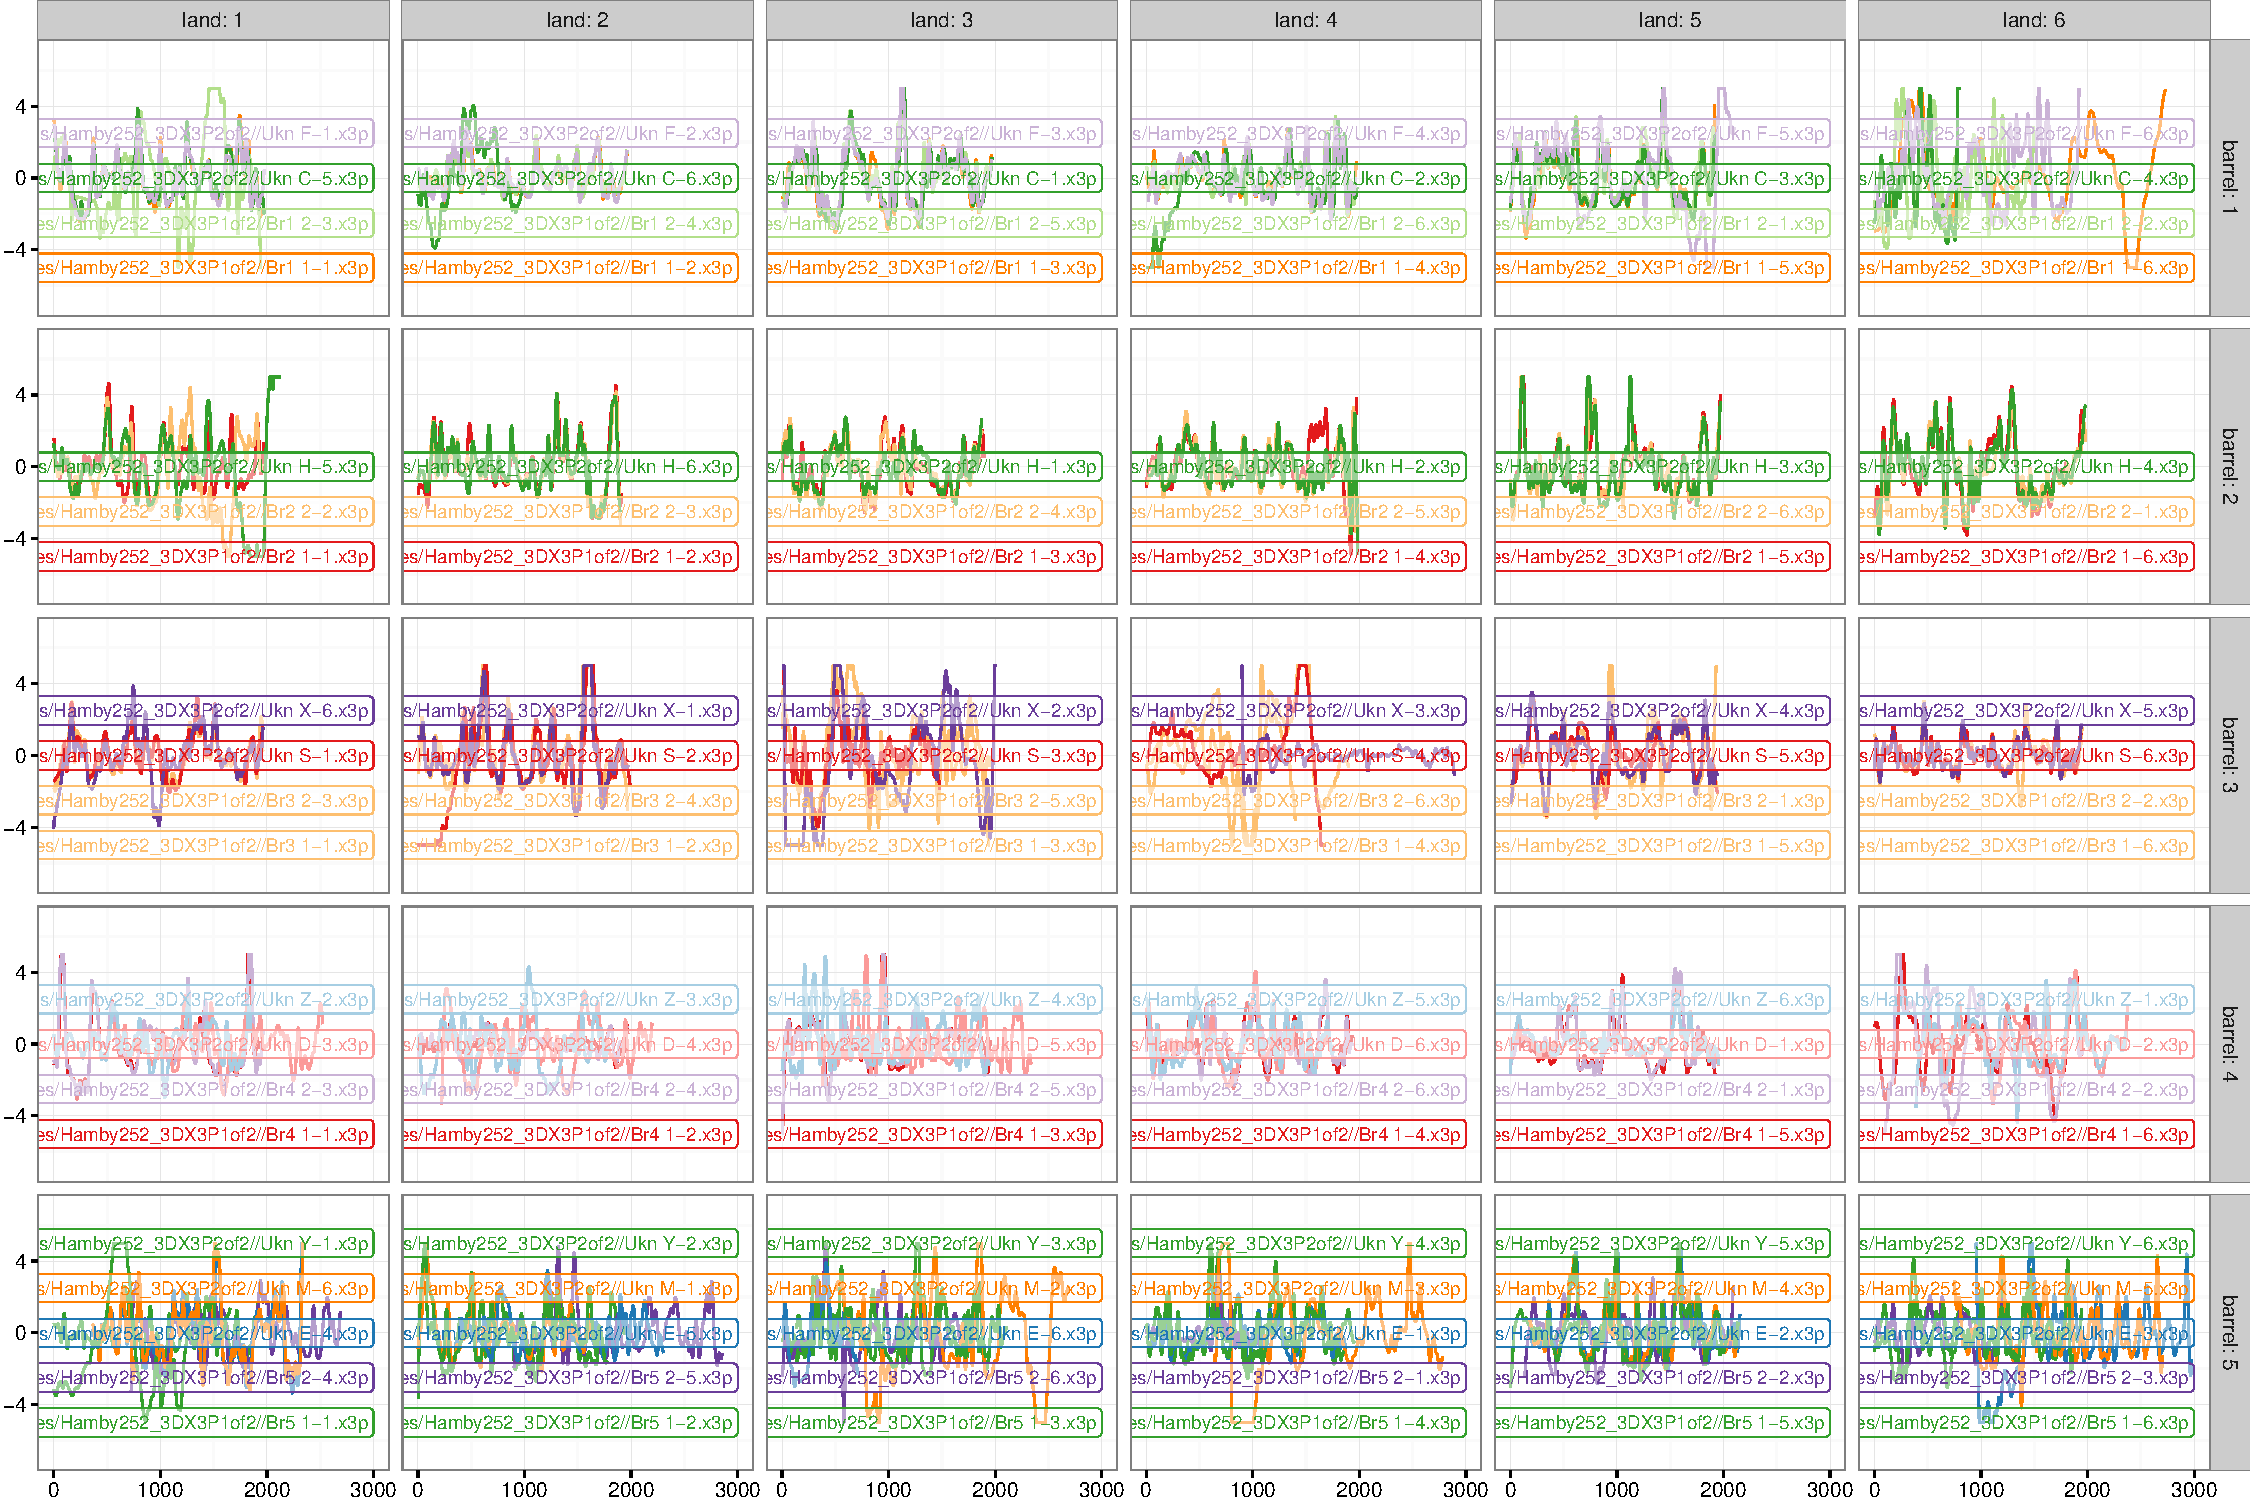
\includegraphics[width=7.5in]{figure/aligned-first-1} 

\end{knitrout}
\caption{\label{fig:aligned}Overview of aligned signatures for all bullet lands for  barrels 1 to 5 of the Hamby study. }
\end{figure}

\begin{figure}[hbtp]
\begin{knitrout}
\definecolor{shadecolor}{rgb}{0.969, 0.969, 0.969}\color{fgcolor}
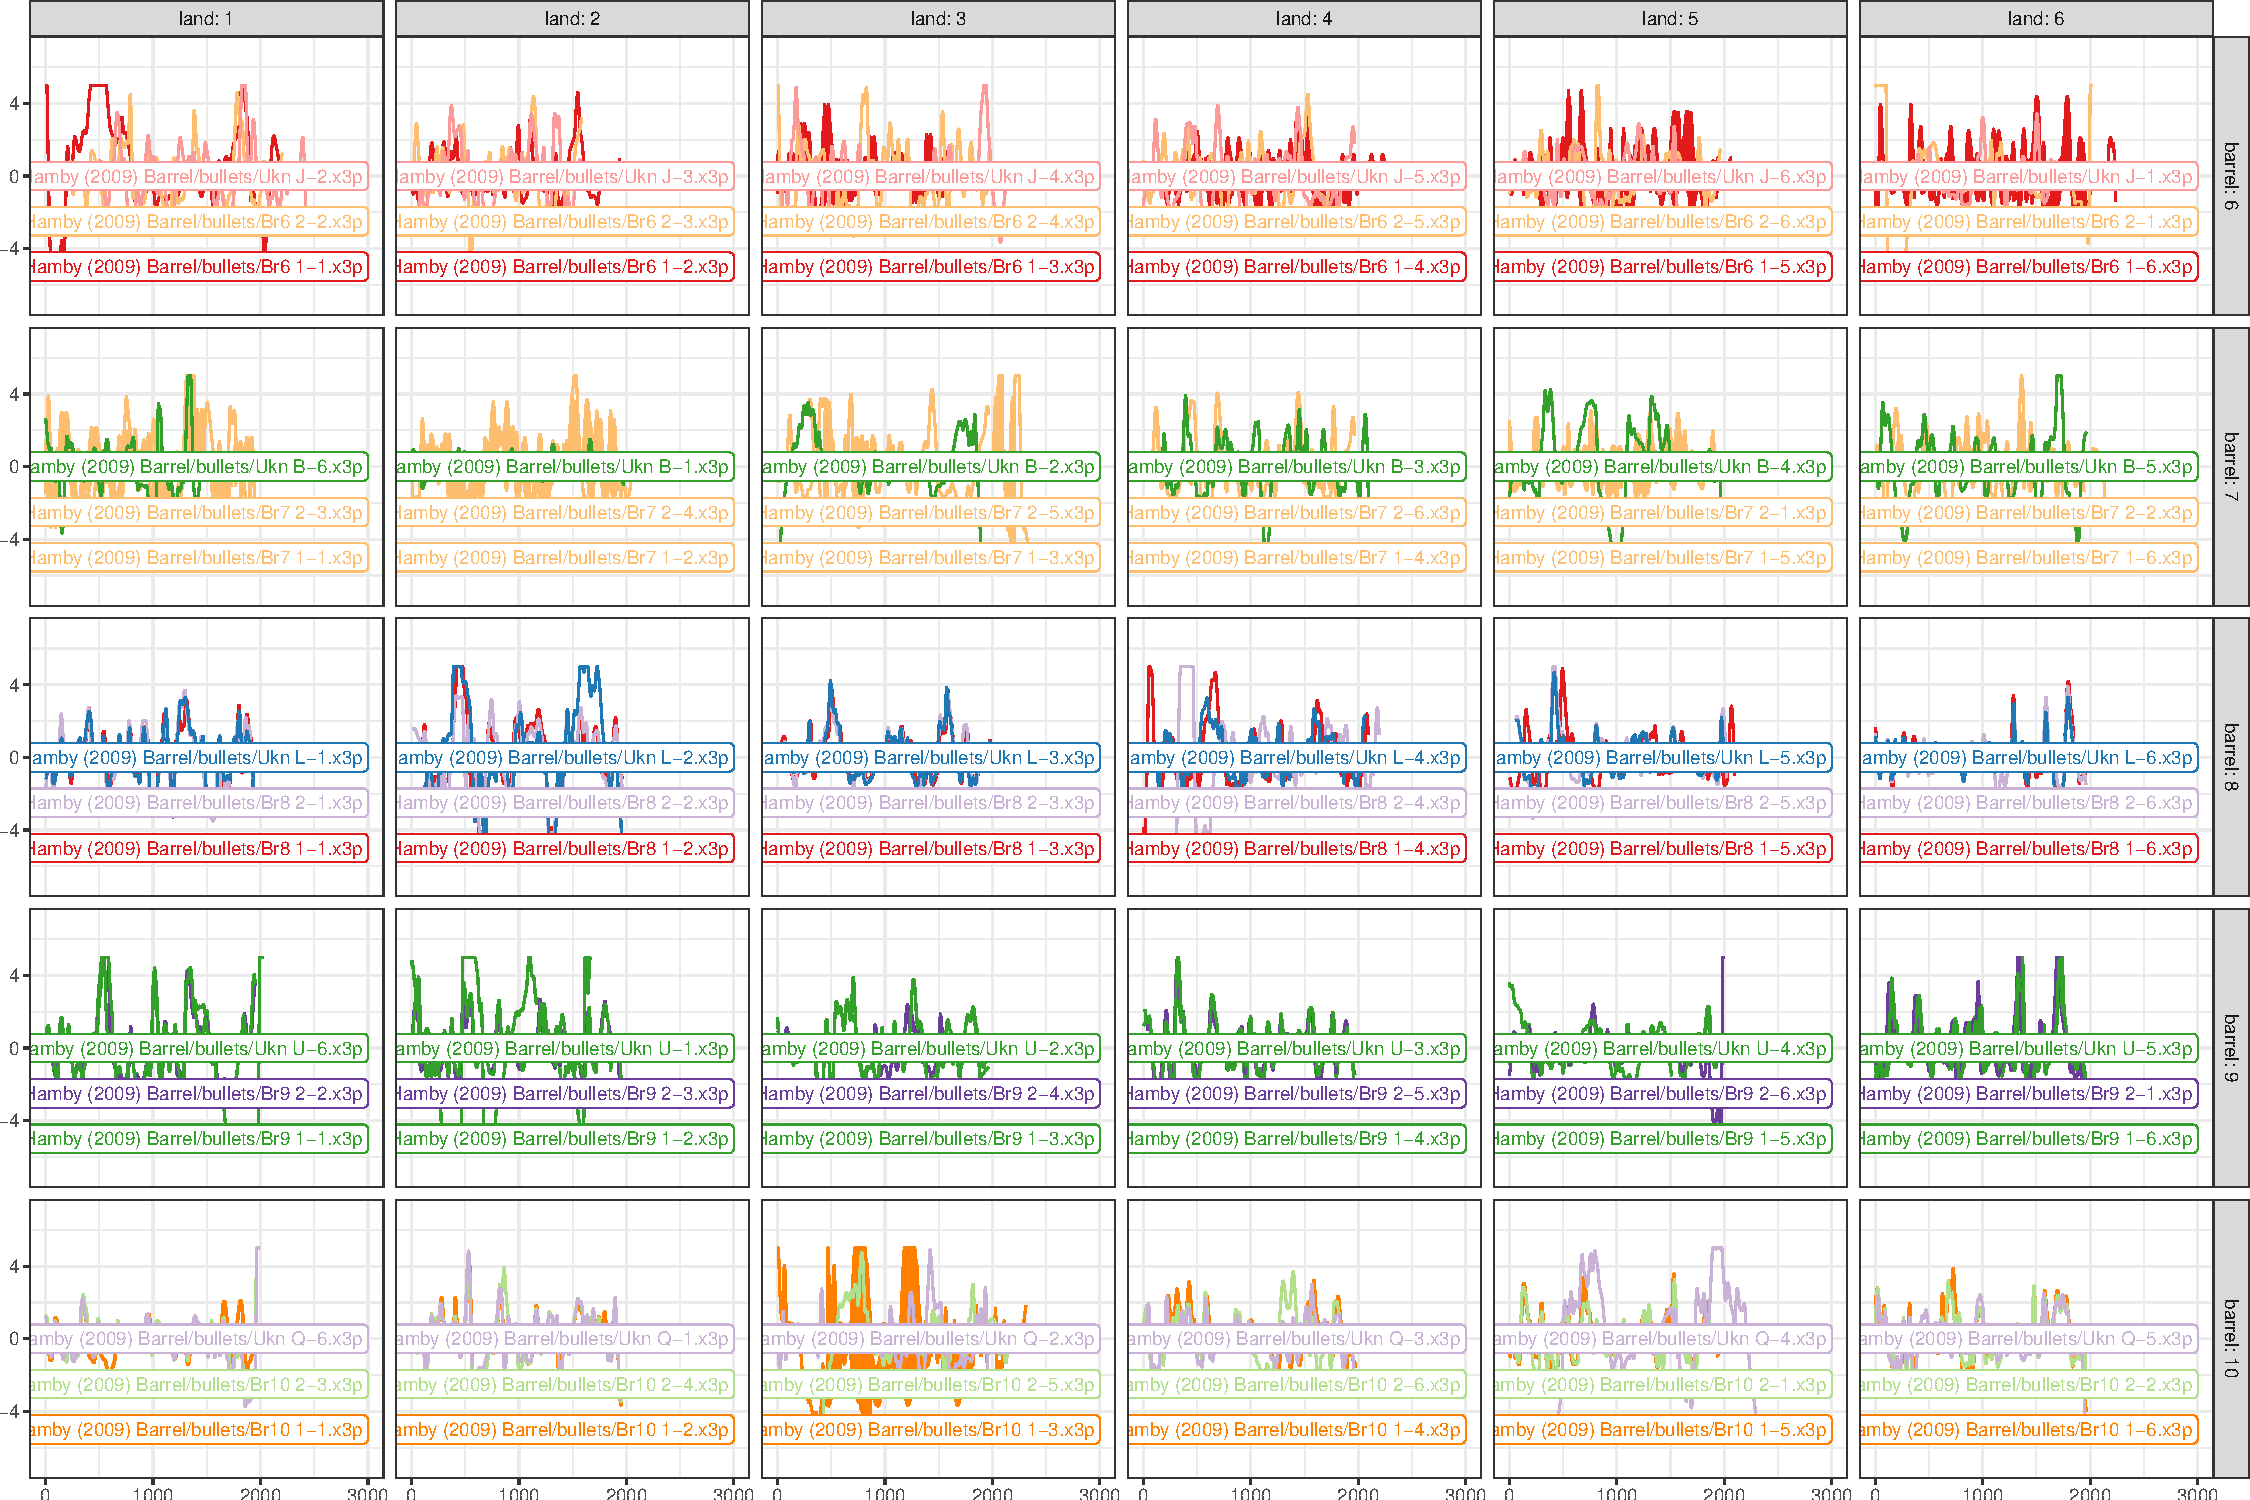
\includegraphics[width=7.5in]{figure/aligned-second-1} 

\end{knitrout}
\caption{\label{fig:aligned-second}Overview of aligned signatures for all bullet lands for  barrels 5 to 10 of the Hamby study. }
\end{figure}
\end{landscape}
\newpage
\section{Table of feature importance}\label{supp:randomforest}
Two random forests were calculated for the Hamby study. For the first random forest only comparisons of bullet lands from known bullets and unknown bullets were used. The second random forest is based on a full comparison of every land with every other land, increasing the number of comparisons from originally 10,384 (10,212 known non-matches and 172 known matches) by another 10,931 comparisons (10,637 known non-matches and 94 known matches). Random forests allow an assessment of variable importance (also called feature importance) as the mean decrease in Gini index when including each variable. 
Table~\ref{tab:importance} shows the results for feature importance for both of these random forests. Importance~1 refers to the smaller subset, Importance~2 is the feature importance derived from the random forest based on all pairwise comparisons. 


\begin{table}[tbhp]
\caption{\label{tab:importance}Table of  features derived from bullet image ordered by importance in predicting matches. Importance is measured in terms of mean decrease in gini index when including the variable in a decision tree. Averages (and standard deviations) for known matches (KM) and known non-matches (KNM) are shown in the last four columns.}
\centering
% latex table generated in R 3.3.2 by xtable 1.8-2 package
% Wed Nov 30 12:56:25 2016
\begin{tabular}{clrrrd{3.2}rd{3.2}}
  \hline
 & Variable & Importance 1 & Importance 2 & KM & (sd) & KNM & (sd).1 \\ 
  \hline
1 & ccf & 87.0 & 134.6 & 0.7 & ( 0.25) & 0.3 & (   0.10) \\ 
  2 & \#matches & 81.9 & 128.3 & 15.5 & ( 7.91) & 4.3 & (   2.51) \\ 
  3 & S & 46.4 & 53.6 & 18.3 & ( 8.95) & 5.5 & (   3.41) \\ 
  4 & \#non-matches & 35.9 & 62.7 & 9.8 & ( 5.80) & 18.8 & (   3.92) \\ 
  5 & D & 26.1 & 45.7 & 1.9 & ( 2.32) & 3.3 & (   1.94) \\ 
  6 & CMS & 15.9 & 25.1 & 8.5 & ( 5.65) & 2.3 & (   1.40) \\ 
  7 & CNMS & 13.3 & 20.9 & 4.8 & ( 4.10) & 10.2 & (   4.35) \\ 
   \hline
\end{tabular}

\end{table}

\bibliographystyle{imsart-nameyear.bst}
%\biboptions{authoryear}
\bibliography{references}


\end{document}
